\documentclass{standalone}
\usepackage{tikz}
\usetikzlibrary{patterns, positioning}


\begin{document}
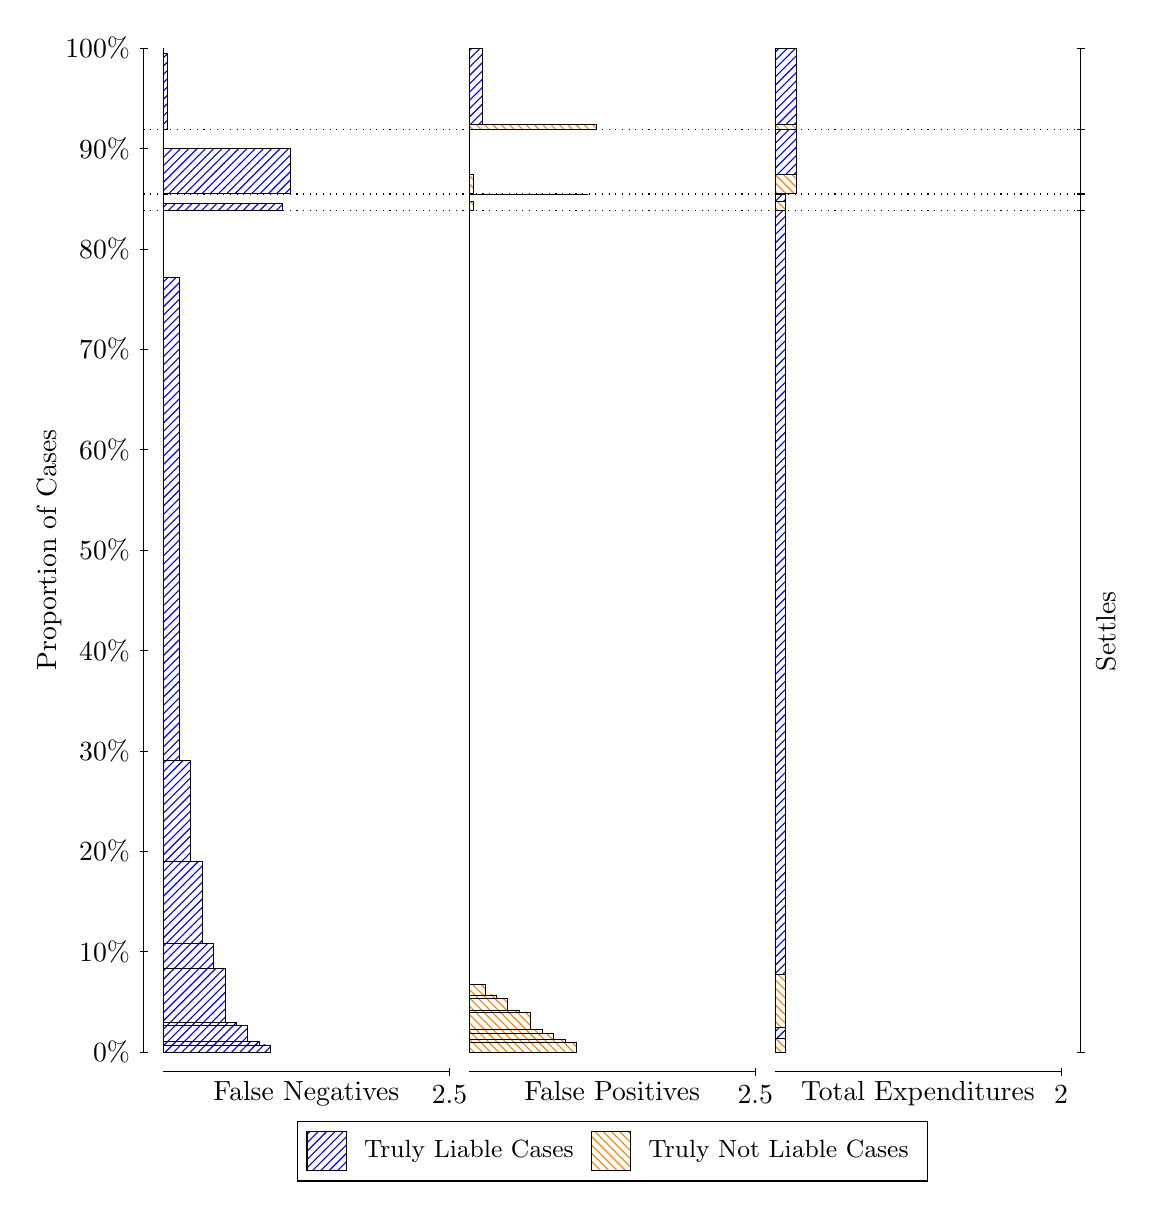
\begin{tikzpicture}
\draw[black, very thin] (1.5,1.75) -- (1.5,14.5);
\node[rotate=90, text=black, anchor=center] at (0.3, 8.125) {Proportion of Cases};
\draw[black, very thin] (1.45,1.75) -- (1.55,1.75);
\node[text=black, anchor=east] at (1.45, 1.75) {0\%};
\draw[black, very thin] (1.45,3.025) -- (1.55,3.025);
\node[text=black, anchor=east] at (1.45, 3.025) {10\%};
\draw[black, very thin] (1.45,4.3) -- (1.55,4.3);
\node[text=black, anchor=east] at (1.45, 4.3) {20\%};
\draw[black, very thin] (1.45,5.575) -- (1.55,5.575);
\node[text=black, anchor=east] at (1.45, 5.575) {30\%};
\draw[black, very thin] (1.45,6.85) -- (1.55,6.85);
\node[text=black, anchor=east] at (1.45, 6.85) {40\%};
\draw[black, very thin] (1.45,8.125) -- (1.55,8.125);
\node[text=black, anchor=east] at (1.45, 8.125) {50\%};
\draw[black, very thin] (1.45,9.4) -- (1.55,9.4);
\node[text=black, anchor=east] at (1.45, 9.4) {60\%};
\draw[black, very thin] (1.45,10.675) -- (1.55,10.675);
\node[text=black, anchor=east] at (1.45, 10.675) {70\%};
\draw[black, very thin] (1.45,11.95) -- (1.55,11.95);
\node[text=black, anchor=east] at (1.45, 11.95) {80\%};
\draw[black, very thin] (1.45,13.225) -- (1.55,13.225);
\node[text=black, anchor=east] at (1.45, 13.225) {90\%};
\draw[black, very thin] (1.45,14.5) -- (1.55,14.5);
\node[text=black, anchor=east] at (1.45, 14.5) {100\%};

\draw[black, very thin] (13.4,1.75) -- (13.4,14.5);
\draw[black, very thin] (13.35,1.75) -- (13.45,1.75);
\node[anchor=west] at (13.35, 1.75) {};
\draw[black, very thin] (13.35,12.437) -- (13.45,12.437);
\node[anchor=west] at (13.35, 12.437) {};
\draw[black, very thin] (13.35,12.644) -- (13.45,12.644);
\node[anchor=west] at (13.35, 12.644) {};
\draw[black, very thin] (13.35,12.652) -- (13.45,12.652);
\node[anchor=west] at (13.35, 12.652) {};
\draw[black, very thin] (13.35,13.464) -- (13.45,13.464);
\node[anchor=west] at (13.35, 13.464) {};
\draw[black, very thin] (13.35,14.5) -- (13.45,14.5);
\node[anchor=west] at (13.35, 14.5) {};

\draw[black, very thin, pattern color=blue, pattern=north east lines] (1.75,1.75) rectangle (3.1125,1.8405);
\draw[black, very thin, pattern color=blue, pattern=north east lines] (1.75,1.8405) rectangle (2.9672,1.8849);
\draw[black, very thin, pattern color=blue, pattern=north east lines] (1.75,1.8849) rectangle (2.8218,2.085);
\draw[black, very thin, pattern color=blue, pattern=north east lines] (1.75,2.085) rectangle (2.6765,2.1222);
\draw[black, very thin, pattern color=blue, pattern=north east lines] (1.75,2.1222) rectangle (2.5312,2.8118);
\draw[black, very thin, pattern color=blue, pattern=north east lines] (1.75,2.8118) rectangle (2.3858,3.1337);
\draw[black, very thin, pattern color=blue, pattern=north east lines] (1.75,3.1337) rectangle (2.2405,4.1751);
\draw[black, very thin, pattern color=blue, pattern=north east lines] (1.75,4.1751) rectangle (2.0952,5.449);
\draw[black, very thin, pattern color=blue, pattern=north east lines] (1.75,5.449) rectangle (1.9498,11.583);
\draw[black, very thin, pattern color=orange, pattern=north west lines] (1.75,11.583) rectangle (1.75,12.437);
\draw[black, very thin, pattern color=blue, pattern=north east lines] (1.75,12.437) rectangle (3.2578,12.529);
\draw[black, very thin, pattern color=orange, pattern=north west lines] (1.75,12.529) rectangle (1.75,12.644);
\draw[black, very thin, pattern color=blue, pattern=north east lines] (1.75,12.644) rectangle (1.8045,12.652);
\draw[black, very thin, pattern color=orange, pattern=north west lines] (1.75,12.652) rectangle (1.75,12.652);
\draw[black, very thin, pattern color=blue, pattern=north east lines] (1.75,12.652) rectangle (3.3668,13.221);
\draw[black, very thin, pattern color=orange, pattern=north west lines] (1.75,13.221) rectangle (1.75,13.464);
\draw[black, very thin, pattern color=blue, pattern=north east lines] (1.75,13.464) rectangle (1.8045,14.438);
\draw[black, very thin, pattern color=orange, pattern=north west lines] (1.75,14.438) rectangle (1.75,14.5);
\draw[black, very thin, pattern color=orange, pattern=north west lines] (5.6333,1.75) rectangle (6.9958,1.8697);
\draw[black, very thin, pattern color=orange, pattern=north west lines] (5.6333,1.8697) rectangle (6.8505,1.9056);
\draw[black, very thin, pattern color=orange, pattern=north west lines] (5.6333,1.9056) rectangle (6.7052,1.9853);
\draw[black, very thin, pattern color=orange, pattern=north west lines] (5.6333,1.9853) rectangle (6.5598,2.0414);
\draw[black, very thin, pattern color=orange, pattern=north west lines] (5.6333,2.0414) rectangle (6.4145,2.256);
\draw[black, very thin, pattern color=orange, pattern=north west lines] (5.6333,2.256) rectangle (6.2692,2.2757);
\draw[black, very thin, pattern color=orange, pattern=north west lines] (5.6333,2.2757) rectangle (6.1238,2.4287);
\draw[black, very thin, pattern color=orange, pattern=north west lines] (5.6333,2.4287) rectangle (5.9785,2.4743);
\draw[black, very thin, pattern color=orange, pattern=north west lines] (5.6333,2.4743) rectangle (5.8332,2.6041);
\draw[black, very thin, pattern color=blue, pattern=north east lines] (5.6333,2.6041) rectangle (5.6333,12.437);
\draw[black, very thin, pattern color=orange, pattern=north west lines] (5.6333,12.437) rectangle (5.6878,12.552);
\draw[black, very thin, pattern color=blue, pattern=north east lines] (5.6333,12.552) rectangle (5.6333,12.644);
\draw[black, very thin, pattern color=orange, pattern=north west lines] (5.6333,12.644) rectangle (7.1412,12.644);
\draw[black, very thin, pattern color=blue, pattern=north east lines] (5.6333,12.644) rectangle (5.6878,12.652);
\draw[black, very thin, pattern color=orange, pattern=north west lines] (5.6333,12.652) rectangle (5.6878,12.896);
\draw[black, very thin, pattern color=blue, pattern=north east lines] (5.6333,12.896) rectangle (5.6333,13.464);
\draw[black, very thin, pattern color=orange, pattern=north west lines] (5.6333,13.464) rectangle (7.2502,13.526);
\draw[black, very thin, pattern color=blue, pattern=north east lines] (5.6333,13.526) rectangle (5.7968,14.5);
\draw[black, very thin, pattern color=orange, pattern=north west lines] (9.5167,1.75) rectangle (9.6529,1.9254);
\draw[black, very thin, pattern color=blue, pattern=north east lines] (9.5167,1.9254) rectangle (9.6529,2.0603);
\draw[black, very thin, pattern color=orange, pattern=north west lines] (9.5167,2.0603) rectangle (9.6529,2.739);
\draw[black, very thin, pattern color=blue, pattern=north east lines] (9.5167,2.739) rectangle (9.6529,12.437);
\draw[black, very thin, pattern color=orange, pattern=north west lines] (9.5167,12.437) rectangle (9.6529,12.552);
\draw[black, very thin, pattern color=blue, pattern=north east lines] (9.5167,12.552) rectangle (9.6529,12.644);
\draw[black, very thin, pattern color=orange, pattern=north west lines] (9.5167,12.644) rectangle (9.6529,12.644);
\draw[black, very thin, pattern color=blue, pattern=north east lines] (9.5167,12.644) rectangle (9.6529,12.652);
\draw[black, very thin, pattern color=orange, pattern=north west lines] (9.5167,12.652) rectangle (9.7892,12.896);
\draw[black, very thin, pattern color=blue, pattern=north east lines] (9.5167,12.896) rectangle (9.7892,13.464);
\draw[black, very thin, pattern color=orange, pattern=north west lines] (9.5167,13.464) rectangle (9.7892,13.526);
\draw[black, very thin, pattern color=blue, pattern=north east lines] (9.5167,13.526) rectangle (9.7892,14.5);
\draw[black, dotted] (1.5,12.437) -- (13.4,12.437);
\draw[black, dotted] (1.5,12.644) -- (13.4,12.644);
\draw[black, dotted] (1.5,12.652) -- (13.4,12.652);
\draw[black, dotted] (1.5,13.464) -- (13.4,13.464);
\draw[black, very thin] (1.75,1.5) -- (5.3833,1.5);
\node[text=black, anchor=north] at (3.5667, 1.5) {False Negatives};
\draw[black, very thin] (5.3833,1.45) -- (5.3833,1.55);
\node[text=black, anchor=north] at (5.3833, 1.45) {2.5};

\draw[black, very thin] (5.6333,1.5) -- (9.2667,1.5);
\node[text=black, anchor=north] at (7.45, 1.5) {False Positives};
\draw[black, very thin] (9.2667,1.45) -- (9.2667,1.55);
\node[text=black, anchor=north] at (9.2667, 1.45) {2.5};

\draw[black, very thin] (9.5167,1.5) -- (13.15,1.5);
\node[text=black, anchor=north] at (11.333, 1.5) {Total Expenditures};
\draw[black, very thin] (13.15,1.45) -- (13.15,1.55);
\node[text=black, anchor=north] at (13.15, 1.45) {2};

\node[text=black, centered, rotate=90] at (13.72, 7.0935) {Settles};





\draw (7.449999999999999,1.5) node[draw=none] (baseCoordinate) {};
\begin{scope}[align=center]
        \matrix[scale=0.5, draw=black, below=0.5cm of baseCoordinate, nodes={draw}, column sep=0.1cm]{
            \node[rectangle, draw, minimum width=0.5cm, minimum height=0.5cm, pattern color=blue, pattern=north east lines] {}; &
            \node[draw=none, font=\small, text=black] (B) {Truly Liable Cases}; &
            \node[rectangle, draw, minimum width=0.5cm, minimum height=0.5cm, pattern color=orange, pattern=north west lines] {}; &
            \node[draw=none, font=\small, text=black] (B) {Truly Not Liable Cases}; \\
            };
\end{scope}

\end{tikzpicture}
\end{document}